\documentclass{article}

\usepackage[a4paper,margin=2cm]{geometry}
\usepackage{graphicx}

%% Hack the caption:
%% http://tex.stackexchange.com/questions/41597/remove-colon-in-the-caption-of-a-figure-without-using-caption-package
\usepackage{etoolbox}
\makeatletter
\patchcmd{\@makecaption}{#1: #2}{\textbf{\Large #1}}{}{}
\makeatother

% !!! For some reason it complains about one of the captions, wants to
% add a $ sign...??

\begin{document}
\pagestyle{empty}

% !!!
% Generated using drawAllNeurons.m
%

\begin{figure}
  \centering
  \fbox{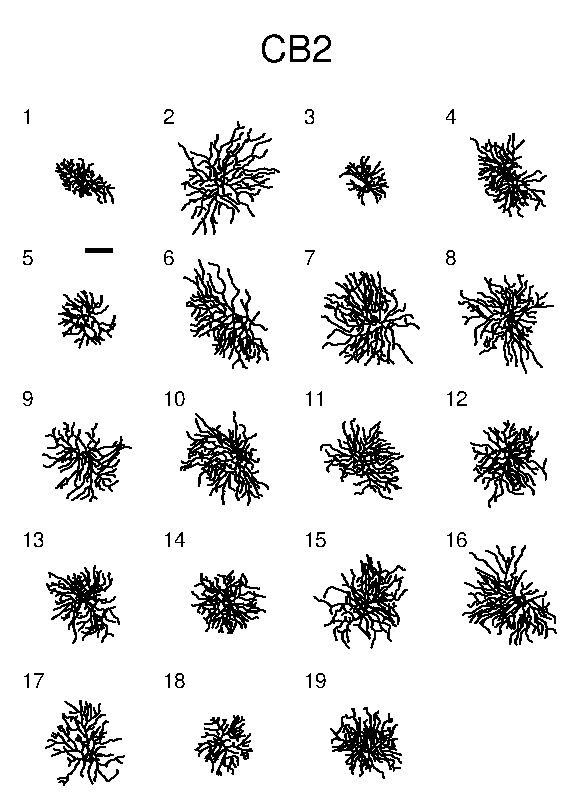
\includegraphics[scale=1.5]{Figures/SupFig1/CB2-all-cells-1.eps}}
  \caption{1. CB2-06142012-cell1-40x
2. CB2-06202012-new
3. CB2-06222012-cell2-b-corrected
4. CB2-07182012-r1-cell1-40x-06zoom-corrected
5. CB2-07182012-r1-cell3-40x-0-corrected
6. CB2-2ears-R1-07062012-cell1-40x-stitch
7. CB2-2ears-R1-07062012-cell3-40x-06zoom
8. CB2-2ears-R1-07062012-cell4-40x-06zoom
9. CB2-2ears-R2-07062012-cell1-40x-06zoom
10. CB2-P62-06252012-40x-stitch
11. CB2-T4-R1-07092012-cell2-40x-stitch
12. CB2-T4-R2-07092012-cell1-40x-stitch
13. CB2-T4-R2-07092012-cell2-40x-07zoom
14. CB2-T4-R2-07092012-cell3-40x-08zoom
15. CB2-nomark-R1-beads-07042012-cell1-40x-06zoom
16. CB2-rightear-R1-beads-07032012-cell1-40x-06zoom
17. CB2-rightear-R2-beads-07032012-cell1-40x-07zoom
18. P61-CB2-06252012-r2-cell1-40x-grey
19. P61-CB2-06252012-r2-cell2-40x-b
}
\end{figure}

\clearpage

\begin{figure}
  \centering
  \fbox{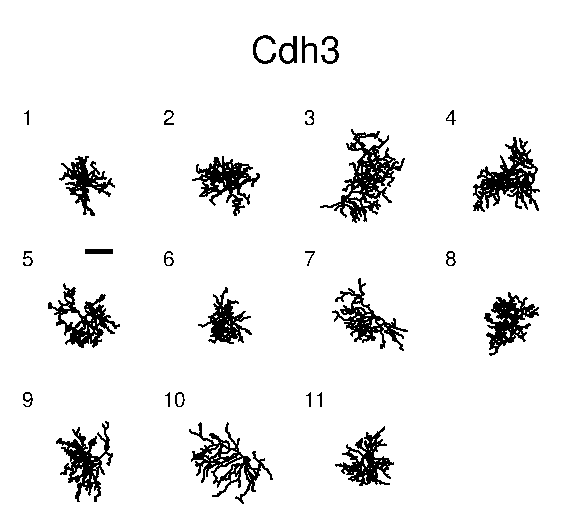
\includegraphics[scale=1.5]{Figures/SupFig1/Cdh3-all-cells-1.eps}}
  \caption{1. Cdh3-06112012-corrected
2. Cdh3-07-17-2012-a2-r2-cell1-40x-0
3. Cdh3-07-17-2012-a2-r2-cell2-40x-0
4. Cdh3-07-18-2012--cell1-40x-0-corrected
5. Cdh3-07-18-2012-a2r2-cell1-40x-0-corrected
6. Cdh3-07-18-2012-a2r2-cell2-40x-corrected
7. Cdh3-07172012-a1r1-cell1-40x-0
8. Cdh3-07172012-a3r3-cell1-40x-09zoom-2
9. Cdh3-07172012-a3r3-cell2-40x-0
10. Cdh3-a3r3-07172012-cell3-40x-0
11. cdh3-03122012-corrected}
\end{figure}

\clearpage

\begin{figure}
  \centering
  \fbox{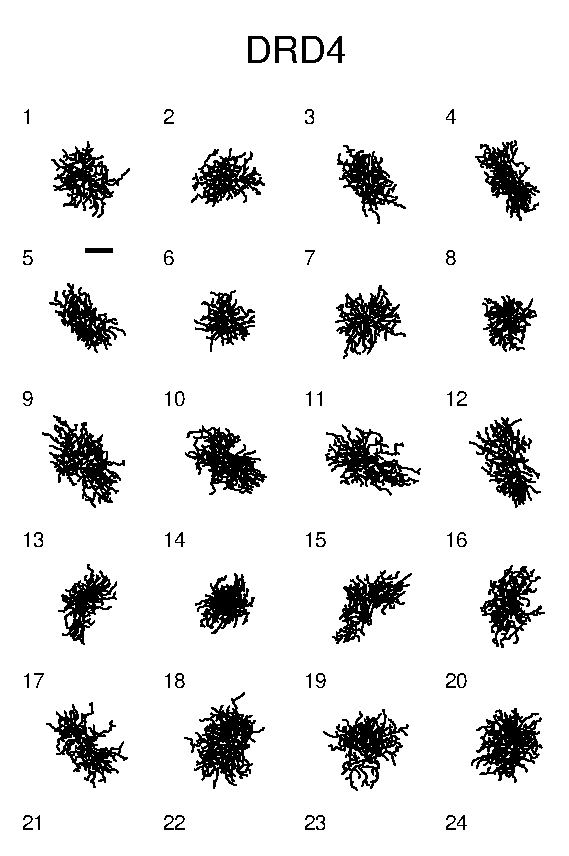
\includegraphics[scale=1.5]{Figures/SupFig1/DRD4-all-cells-1.eps}}
  \caption{1. DRD4-07142012-r2-cell1-40x-0
2. DRD4-07142012-r2-cell2-40x-0
3. DRD4-albino-leftearclip-righteye-control-06022013-cell1-40x-07zoom
4. DRD4-albino-leftearclip-righteye-control-06022013-cell2-40x-07zoom
5. DRD4-albino-leftearclip-righteye-control-06022013-cell3-40x-0_Subset
6. DRD4-albino-leftearclip-righteye-control-06022013-cell4-40x-09zoom
7. DRD4-albino-leftearclip-righteye-control-06022013-cell5-40x-08zoom
8. DRD4-albino-leftearclip-righteye-control-06022013-cell6-40x
9. DRD4-brown-noearclip-righteye-control-06012013-cell1-40x-06zoom
10. DRD4-brown-noearclip-righteye-control-06012013-cell2-40x-07zoom
11. DRD4-brown-noearclip-righteye-control-06012013-cell3-40x-06zoom
12. DRD4-brown-noearclip-righteye-control-06012013-cell4-40x-tile
13. DRD4-noearclip-righteye-control-06012013-cell1-40x-07zoom
14. DRD4-noearclip-righteye-control-06012013-cell2-40x-09zoom
15. DRD4-noearclip-righteye-control-06012013-cell4-40x-07zoom
16. DRD4-noearclip-righteye-control-06012013-cell5-40x-07zoom
17. DRD4-noearclip-righteye-control-06012013-cell6-40x-07zoom
18. P25-DRD4-07142012-r1-c1-40x-06zoom-grey-corrected
19. P25-DRD4-07142012-r1-c2-40x-07zoom
20. P25-DRD4-07142012-r1-cells3
21. P25-DRD4-07142012-r1-cells4
22. P30-DRD4-07102012-a1r1-cell2-40x-0
23. P30-DRD4-07102012-a1r3-cell1-40x-0
24. P30-DRD4-07102012-a2r1-cell1-40x-07zoom}
25. P30-DRD4-07102012-a2r2-cell1-40x-08zoom-grey
26. P30-DRD4-0710210-a1r1-cell1-40x-08zoom
\end{figure}

\clearpage

\begin{figure}
  \centering
  \fbox{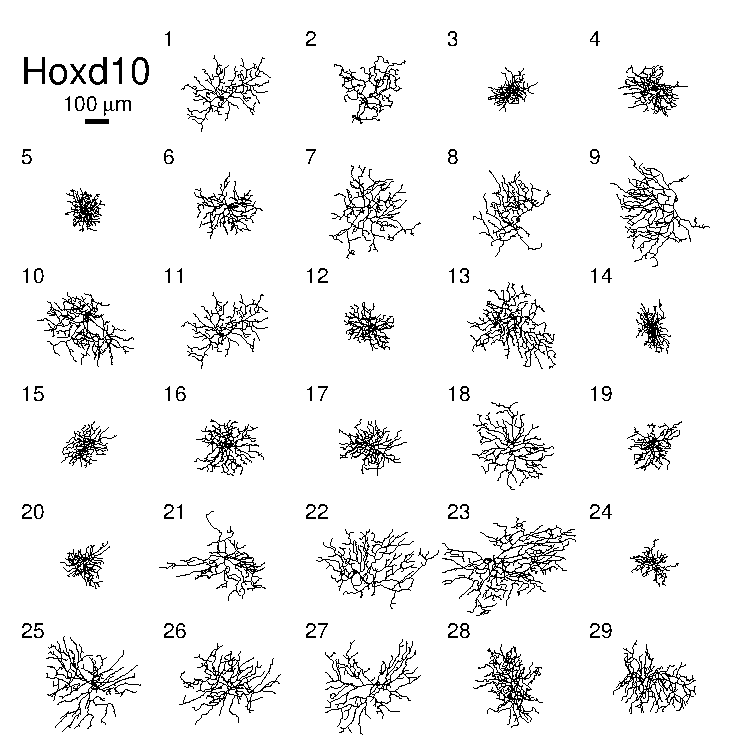
\includegraphics[scale=1.5]{Figures/SupFig1/Hoxd10-all-cells-1.eps}}
  \caption{1. Hoxd10-02242012
2. Hoxd10-03122012-c1-corrected
3. Hoxd10-03122012
4. Hoxd10-03132012-r1c3-corrected
5. Hoxd10-04022012
6. Hoxd10-04032012-corrected
7. Hoxd10-04292013-leftear-righteyecontrol-cell3-40x-tile_Stitch
8. Hoxd10-04292013-rightear-righteyecontrol-cell1-40x-tile_Stitch
9. Hoxd10-04292013-rightear-righteyecontrol-cell2-40x-tile
10. Hoxd10-06062012-c2-corrected
11. Hoxd10-06082012-c1-corrected
12. Hoxd10-06112012-corrected
13. Hoxd10-07022012-retina1-cell3-40x-stitch
14. Hoxd10-bothears-righteyecontrol-04302013-40x-cell1-09zoom
15. Hoxd10-bothears-righteyecontrol-04302013-40x-cell2-09zoom
16. Hoxd10-leftear-righteyecontrol-04292013-40x-cell1-07zoom
17. Hoxd10-leftear-righteyecontrol-04292013-40x-cell2-07zoom
18. Hoxd10-none-righteyecontrol-04292013-40x-cell1-stitch
19. Hoxd10-none-righteyecontrol-04292013-40x-cell2-09zoom
20. Hoxd10-none-righteyecontrol-04292013-40x-cell3
21. Hoxd10-none-righteyecontrol-04292013-40x-cell4-zoom07-stitch
22. Hoxd10-none-righteyecontrol-04292013-40x-cell5-stitch
23. P25-Hoxd1007132012-r2-25x-06zoom
24. P25Hoxd10-07132012-retina1-40x-stitch
25. P82-Hoxd10-retina2-cell4-07022012
26. P82-Hoxd10-retina3-07022012-cell5-40x-stitch
27. P82-Hoxd10-retina3-07022012-cell6-40x-stitch
28. hoxd10-04302013-bothears-righteyecontrol-cell3-40x-06zoom
29. hoxd10-04302013-bothears-righteyecontrol-cell4-40x-06zoom}
\end{figure}

\clearpage

\begin{figure}
  \centering
  \fbox{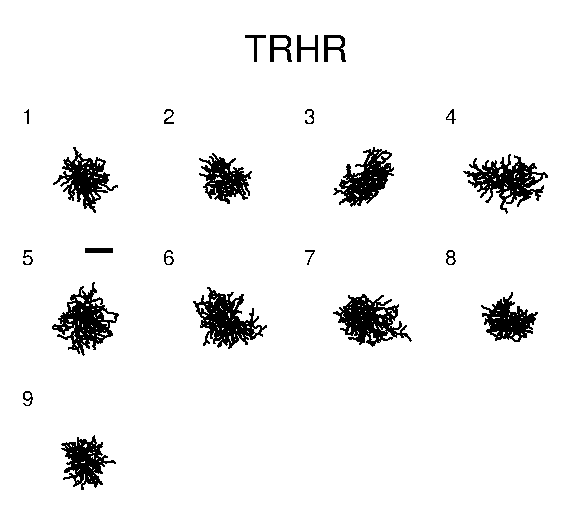
\includegraphics[scale=1.5]{Figures/SupFig1/TRHR-all-cells-1.eps}}
  \caption{1. P32TRHR-02232012-A1R1-40x-stitch
2. P34TRHR-02242012-R1C2-40x
3. P40-TRHR-03222012-r2c2-40x
4. TRHR-07182012-a1r1-cell1-40x-0
5. TRHR-07182012-a1r1-cell2-40x-0.8zoom
6. TRHR-07182012-a1r2-40x-08zoom
7. TRHR-07182012-a1r2-cell2-40x-07zoom
8. TRHR-r1-01252012-40x
9. trhr-04032012-corrected}
\end{figure}

\clearpage


% To generate figures:
% drawAllNeuronsSide.m

\begin{figure}
  \centering
  \fbox{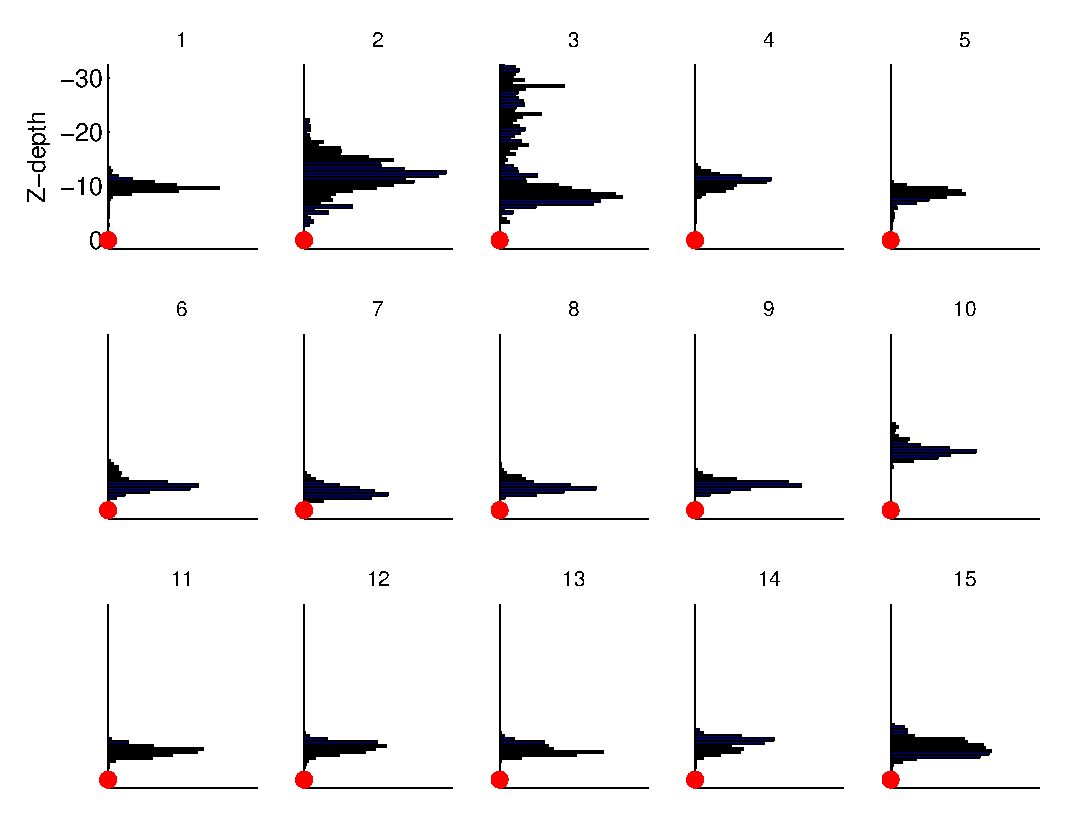
\includegraphics[scale=1]{Figures/SupFig2/CB2-stratification-depth-1}}
  \caption{}
\end{figure}

\clearpage

\begin{figure}
  \centering
  \fbox{\includegraphics[scale=1]{Figures/SupFig2/CB2-stratification-depth-9}}
  \caption{}
\end{figure}

\clearpage

\begin{figure}
  \centering
  \fbox{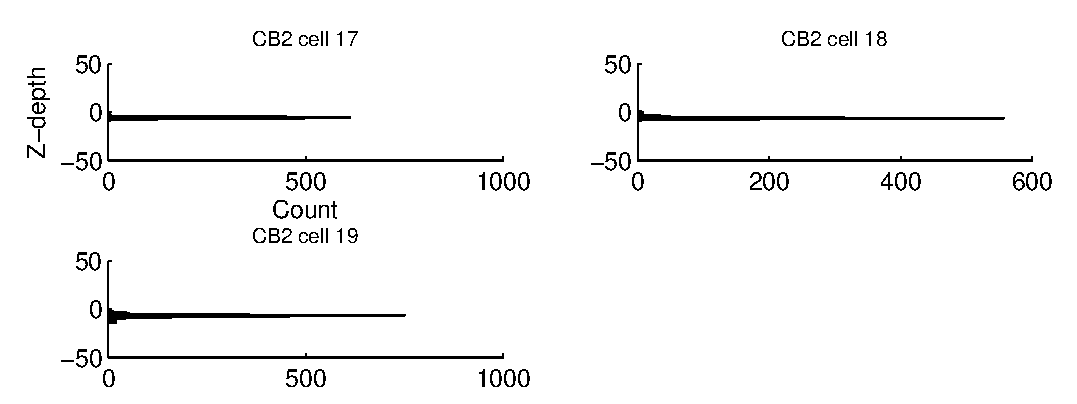
\includegraphics[scale=1]{Figures/SupFig2/CB2-stratification-depth-17}}
  \caption{}
\end{figure}

\clearpage

\begin{figure}
  \centering
  \fbox{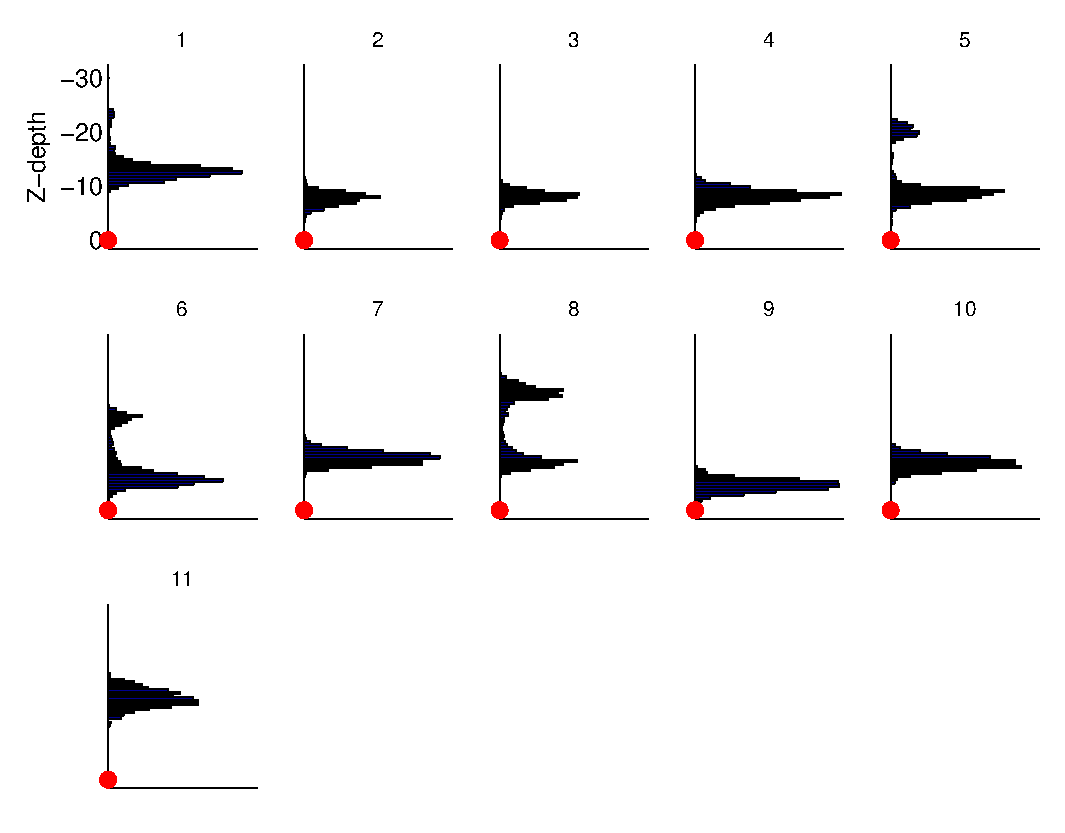
\includegraphics[scale=1]{Figures/SupFig2/Cdh3-stratification-depth-1}}
  \caption{}
\end{figure}

\clearpage

\begin{figure}
  \centering
  \fbox{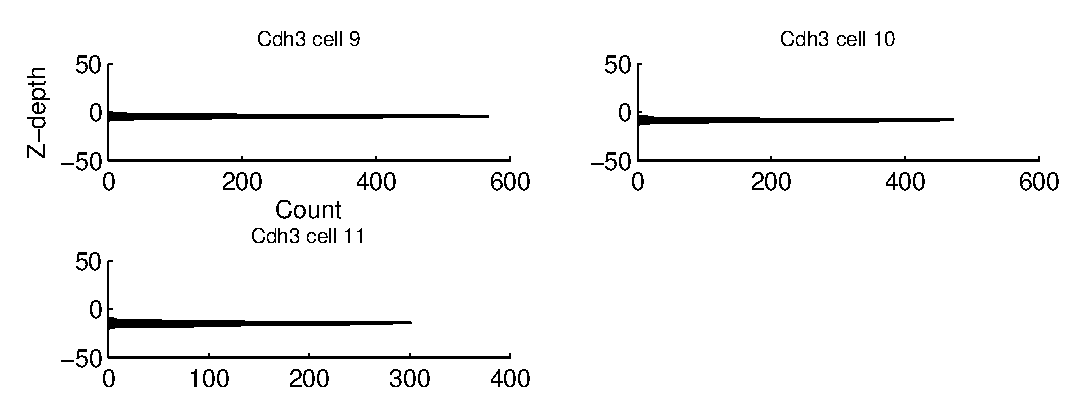
\includegraphics[scale=1]{Figures/SupFig2/Cdh3-stratification-depth-9}}
  \caption{}
\end{figure}

\clearpage

\begin{figure}
  \centering
  \fbox{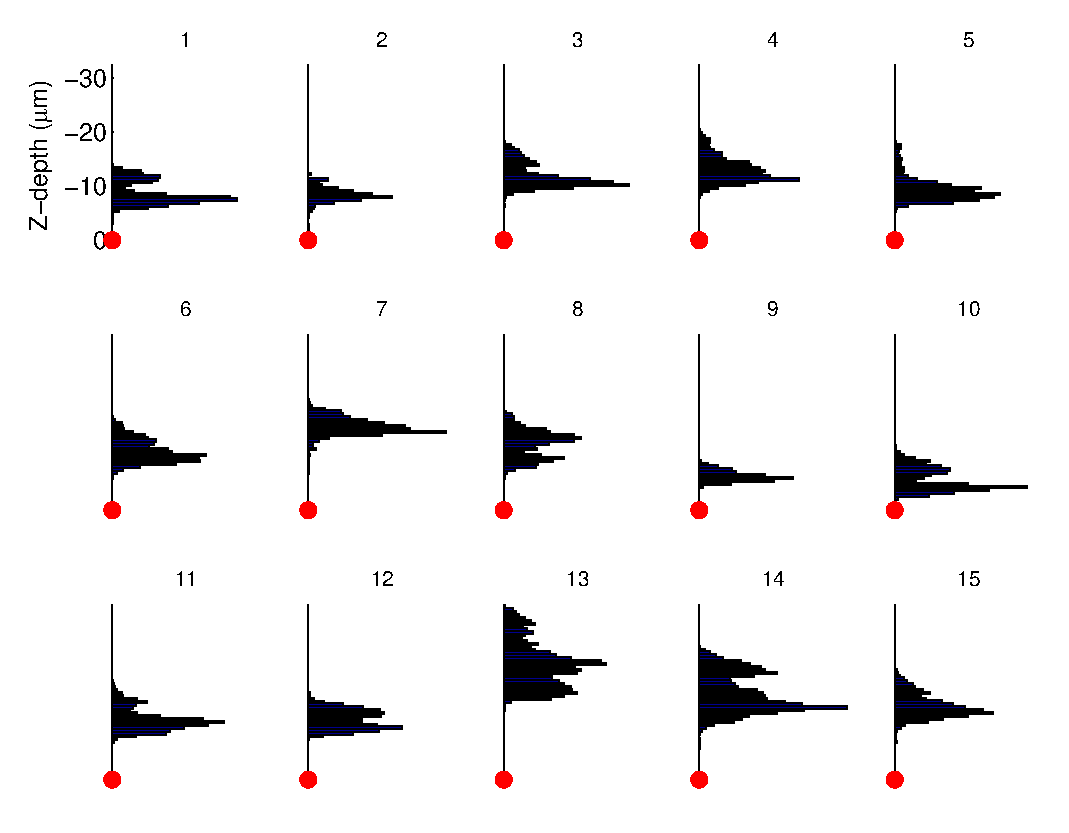
\includegraphics[scale=1]{Figures/SupFig2/DRD4-stratification-depth-1}}
  \caption{}
\end{figure}

\clearpage

\begin{figure}
  \centering
  \fbox{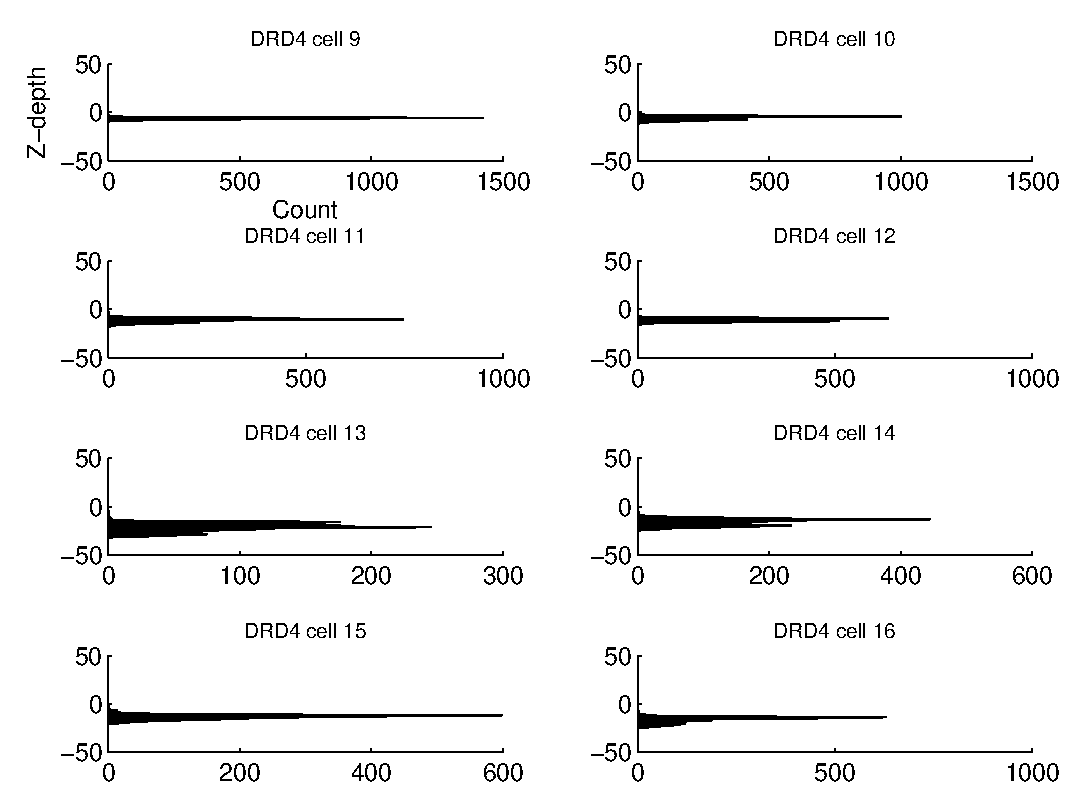
\includegraphics[scale=1]{Figures/SupFig2/DRD4-stratification-depth-9}}
  \caption{}
\end{figure}

\clearpage

\begin{figure}
  \centering
  \fbox{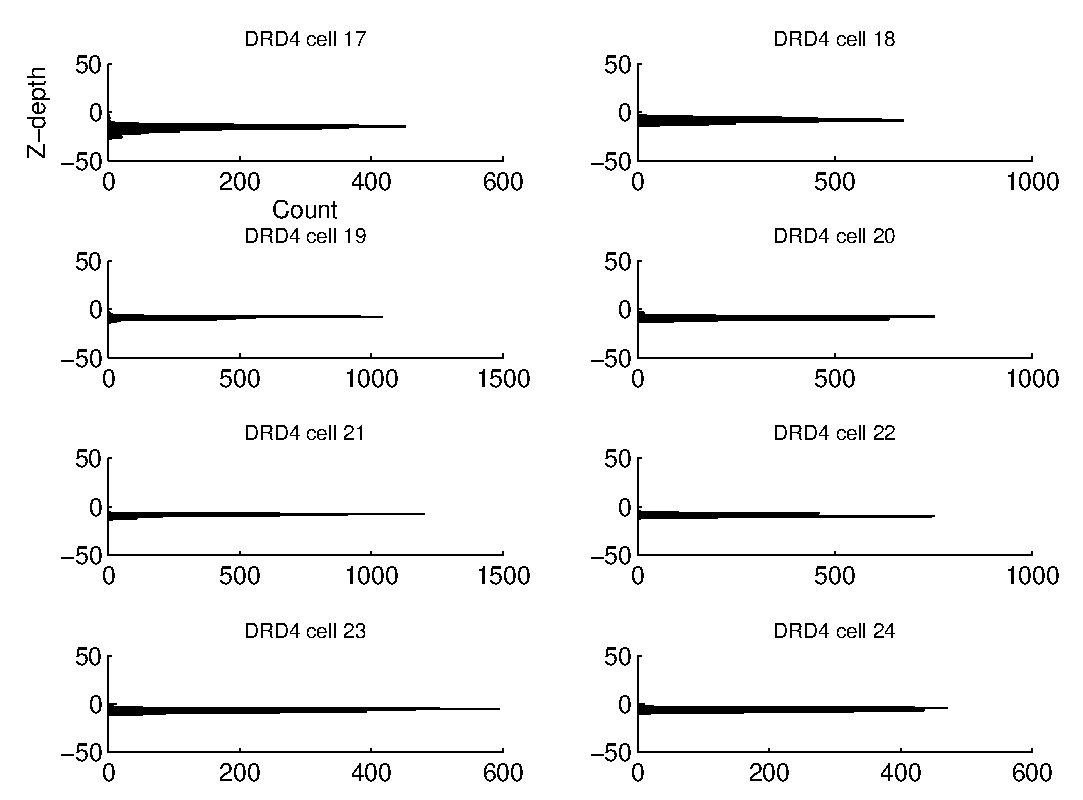
\includegraphics[scale=1]{Figures/SupFig2/DRD4-stratification-depth-17}}
  \caption{}
\end{figure}

\clearpage

\begin{figure}
  \centering
  \fbox{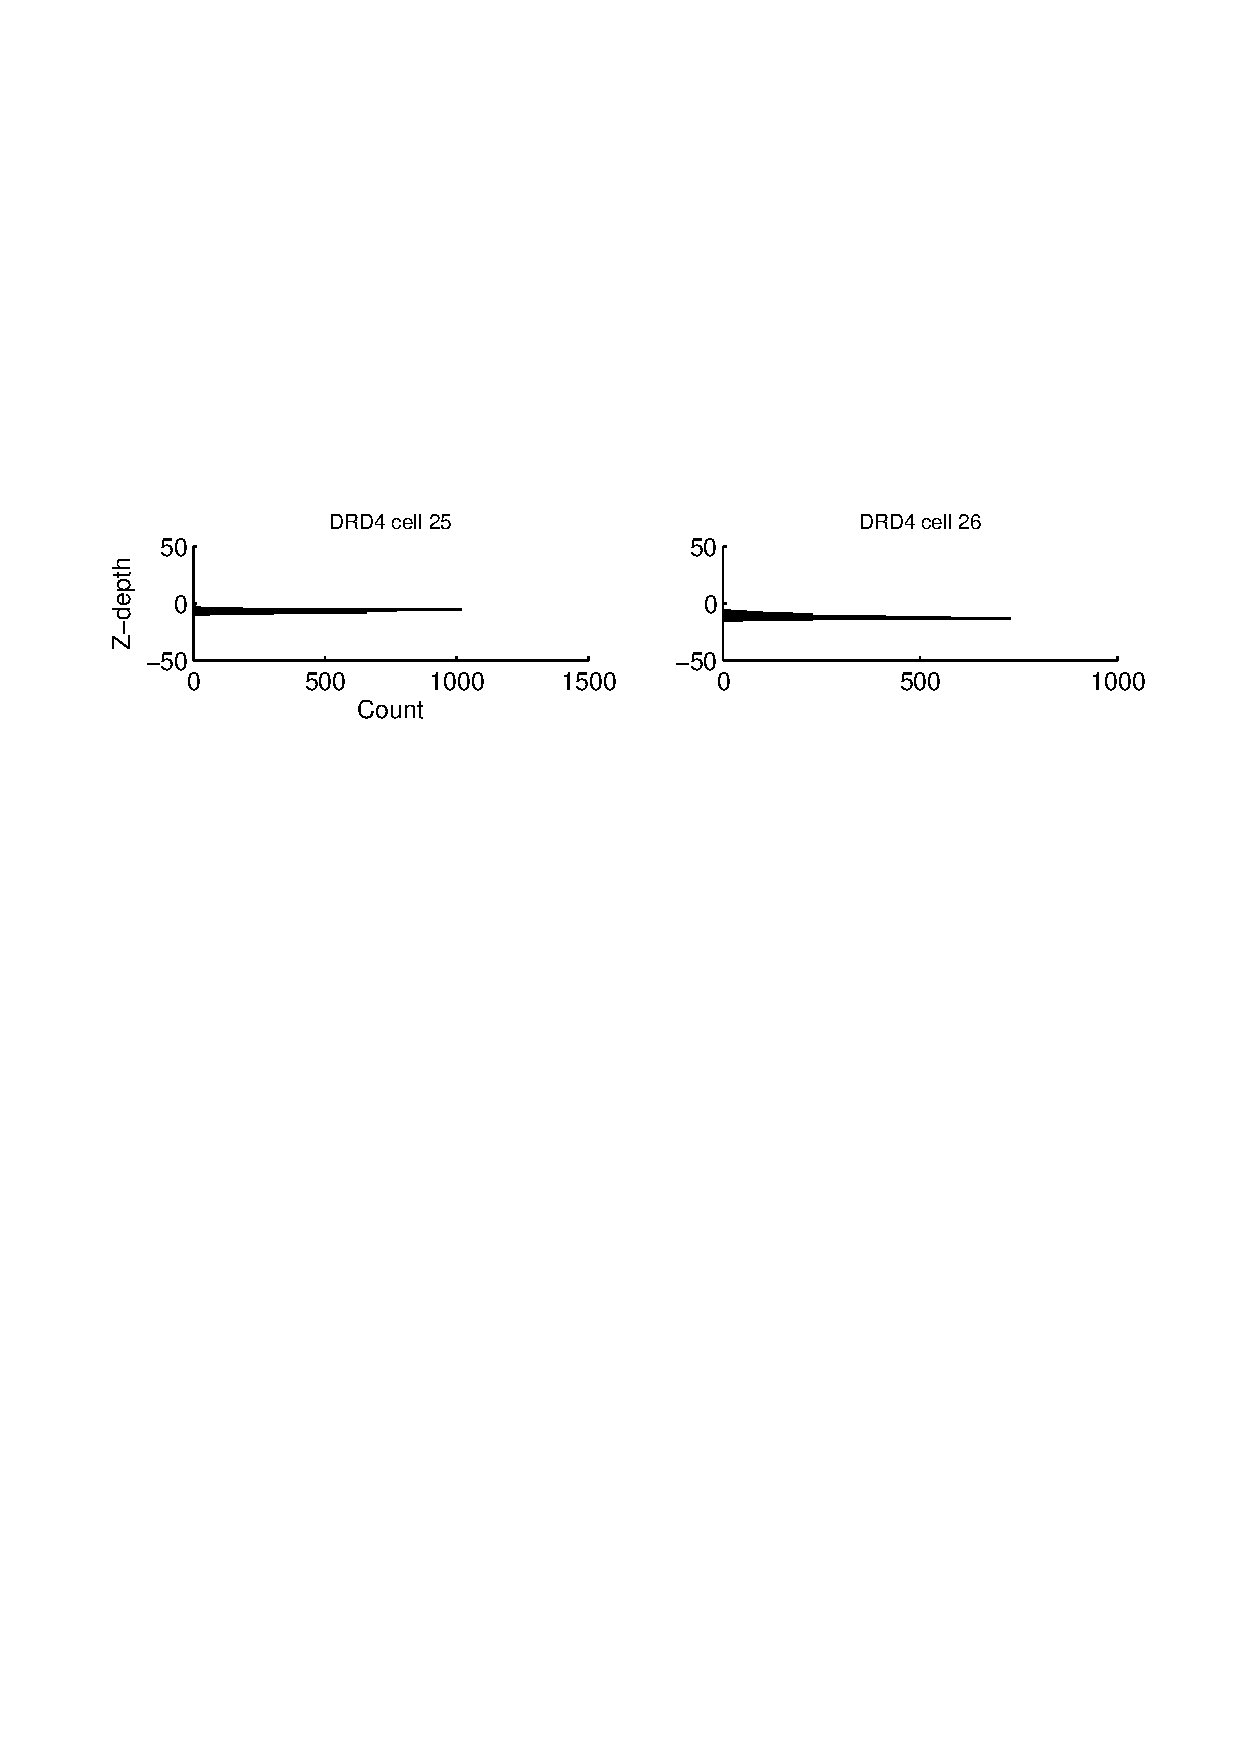
\includegraphics[scale=1]{Figures/SupFig2/DRD4-stratification-depth-25}}
  \caption{}
\end{figure}

\clearpage

\begin{figure}
  \centering
  \fbox{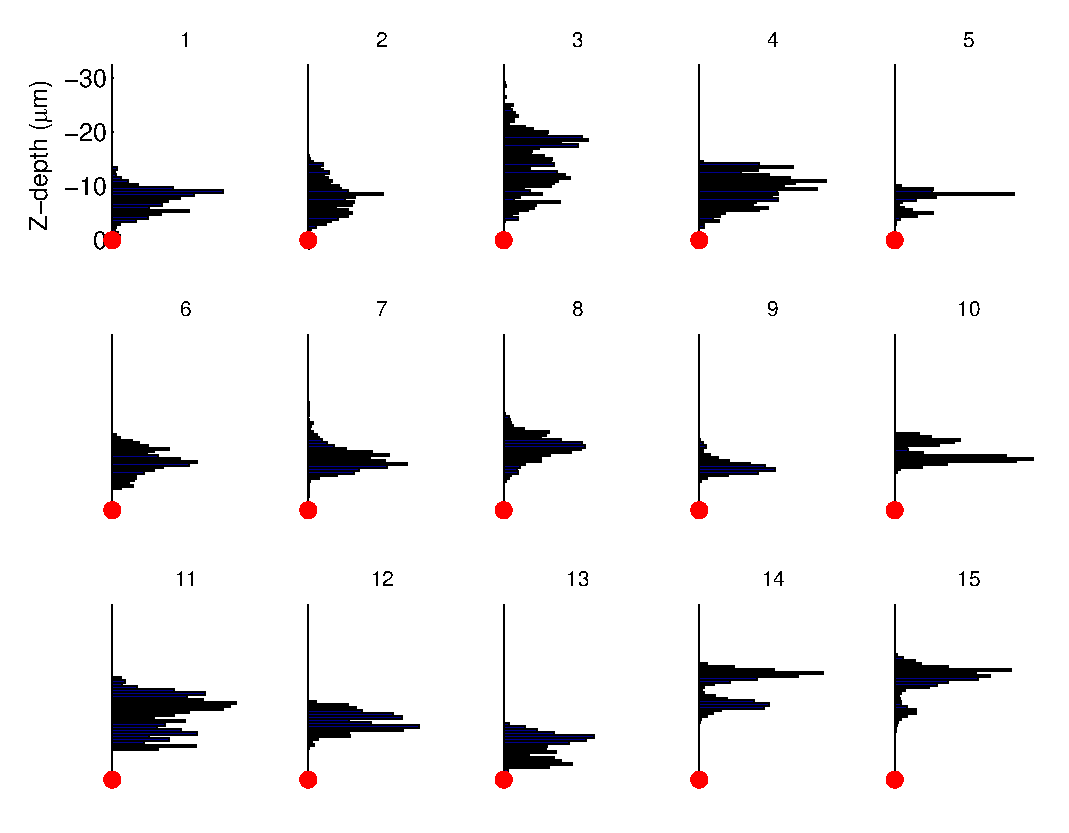
\includegraphics[scale=1]{Figures/SupFig2/Hoxd10-stratification-depth-1}}
  \caption{}
\end{figure}

\clearpage

\begin{figure}
  \centering
  \fbox{\includegraphics[scale=1]{Figures/SupFig2/Hoxd10-stratification-depth-9}}
  \caption{}
\end{figure}

\clearpage

\begin{figure}
  \centering
  \fbox{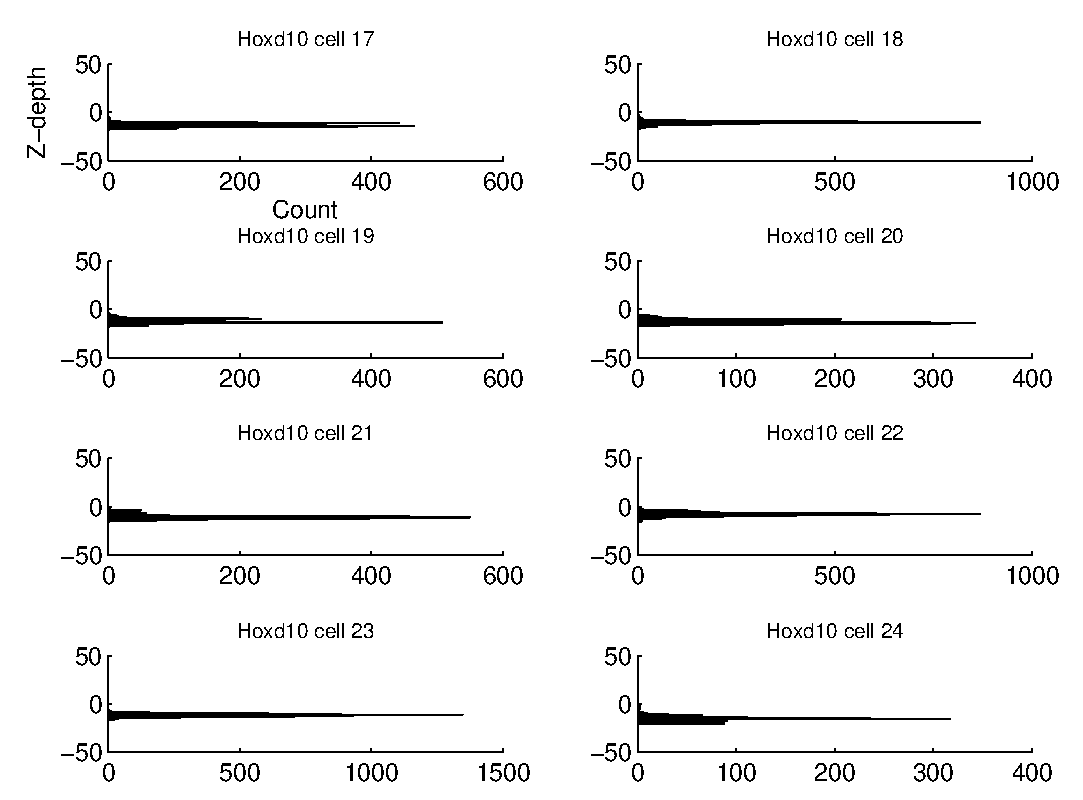
\includegraphics[scale=1]{Figures/SupFig2/Hoxd10-stratification-depth-17}}
  \caption{}
\end{figure}

\clearpage

\begin{figure}
  \centering
  \fbox{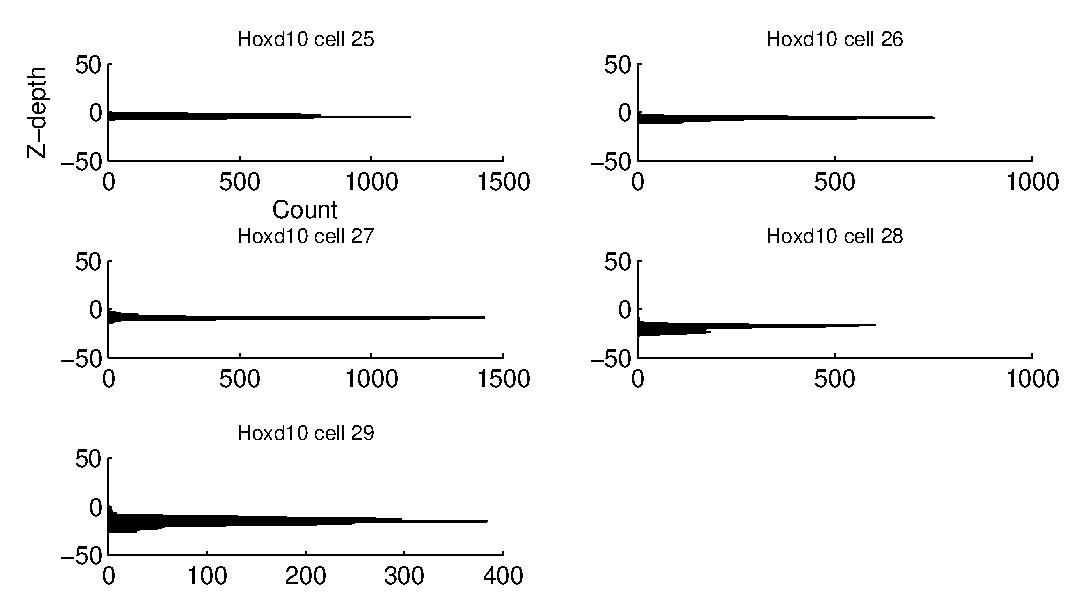
\includegraphics[scale=1]{Figures/SupFig2/Hoxd10-stratification-depth-25}}
  \caption{}
\end{figure}

\clearpage

\begin{figure}
  \centering
  \fbox{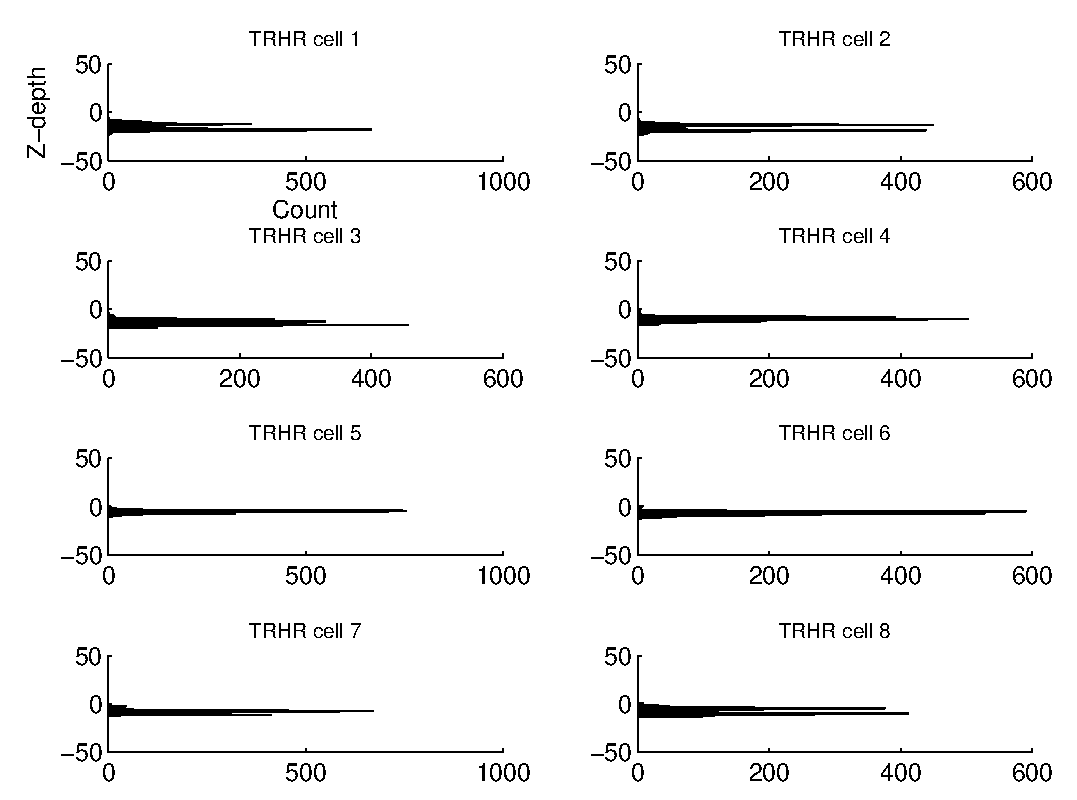
\includegraphics[scale=1]{Figures/SupFig2/TRHR-stratification-depth-1}}
  \caption{}
\end{figure}

\clearpage

\begin{figure}
  \centering
  \fbox{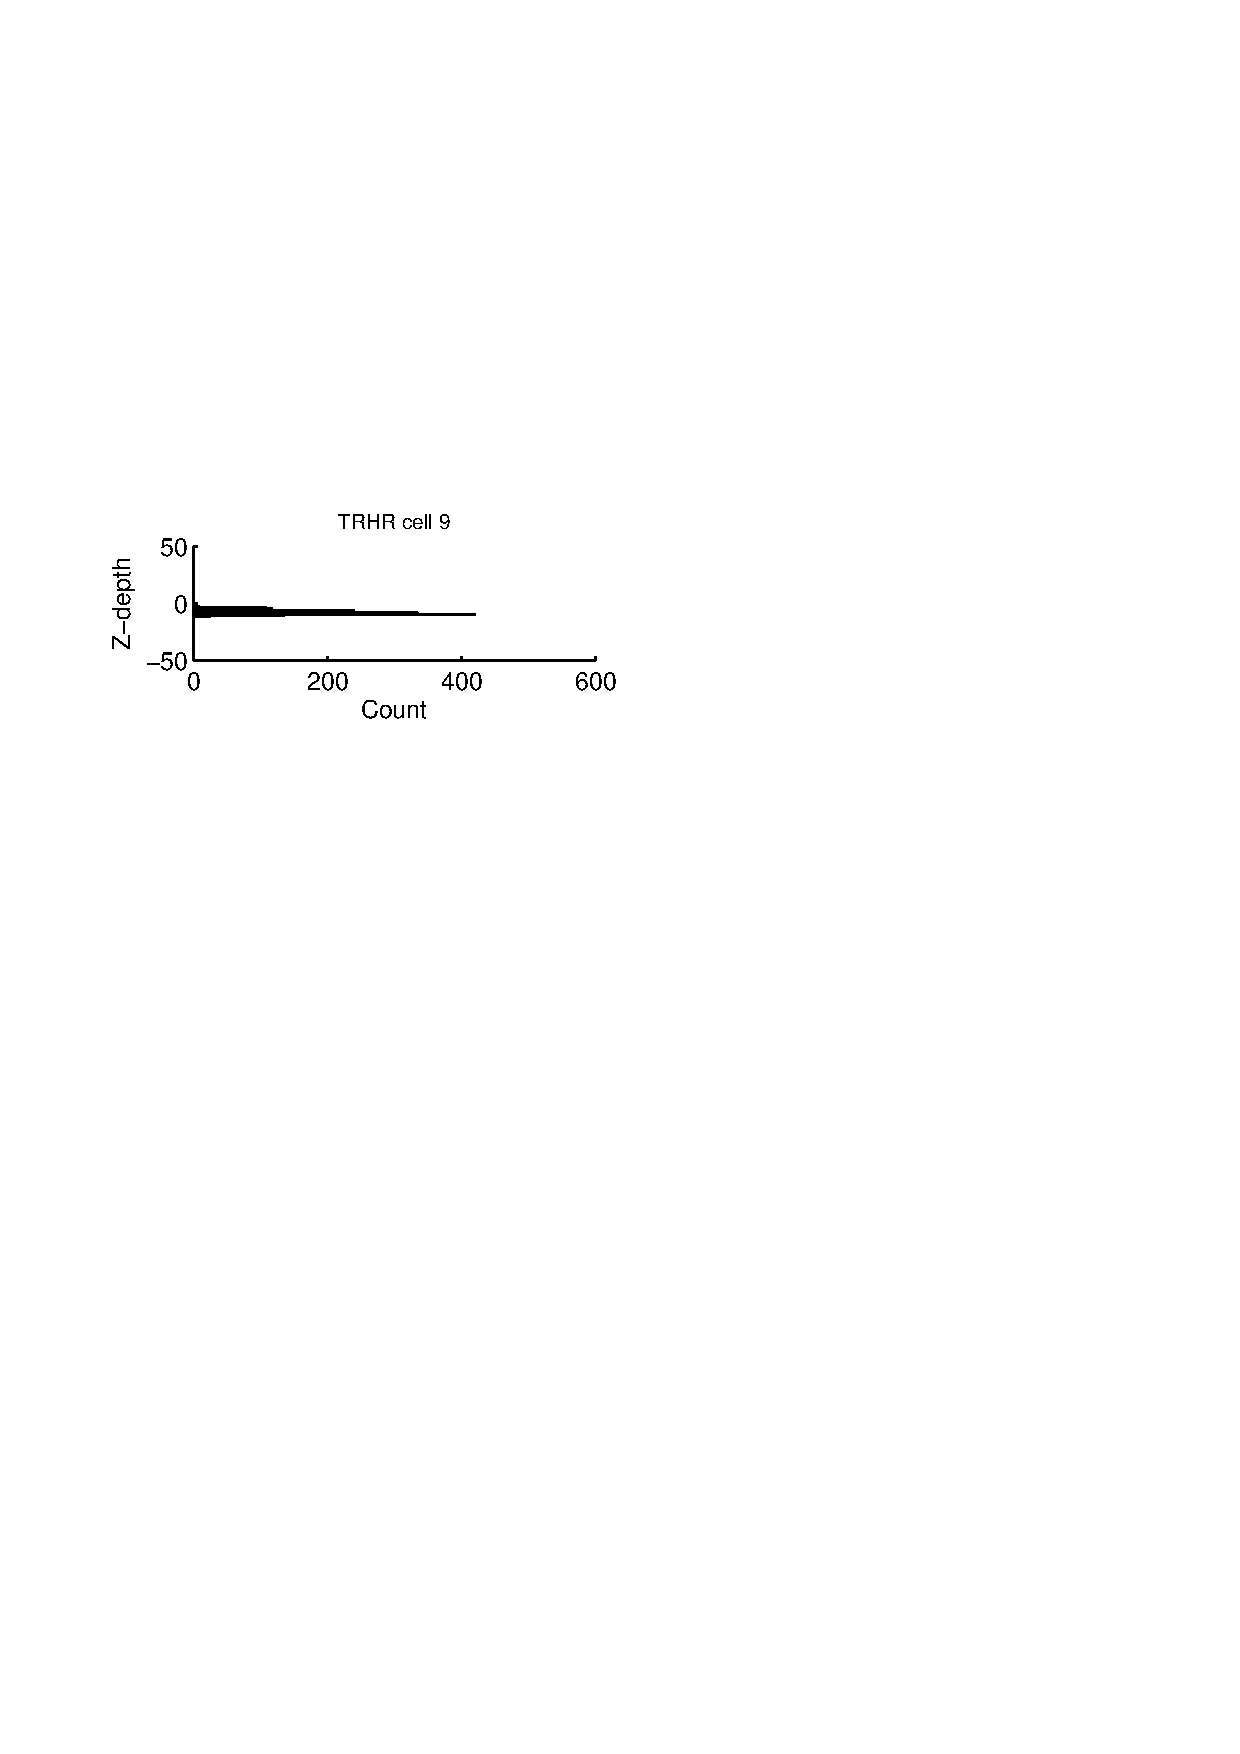
\includegraphics[scale=1]{Figures/SupFig2/TRHR-stratification-depth-9}}
  \caption{}
\end{figure}

\clearpage

% To generate figures:
% plotAllFeaturesForSupplementary.m

\begin{figure}
  \centering
  \fbox{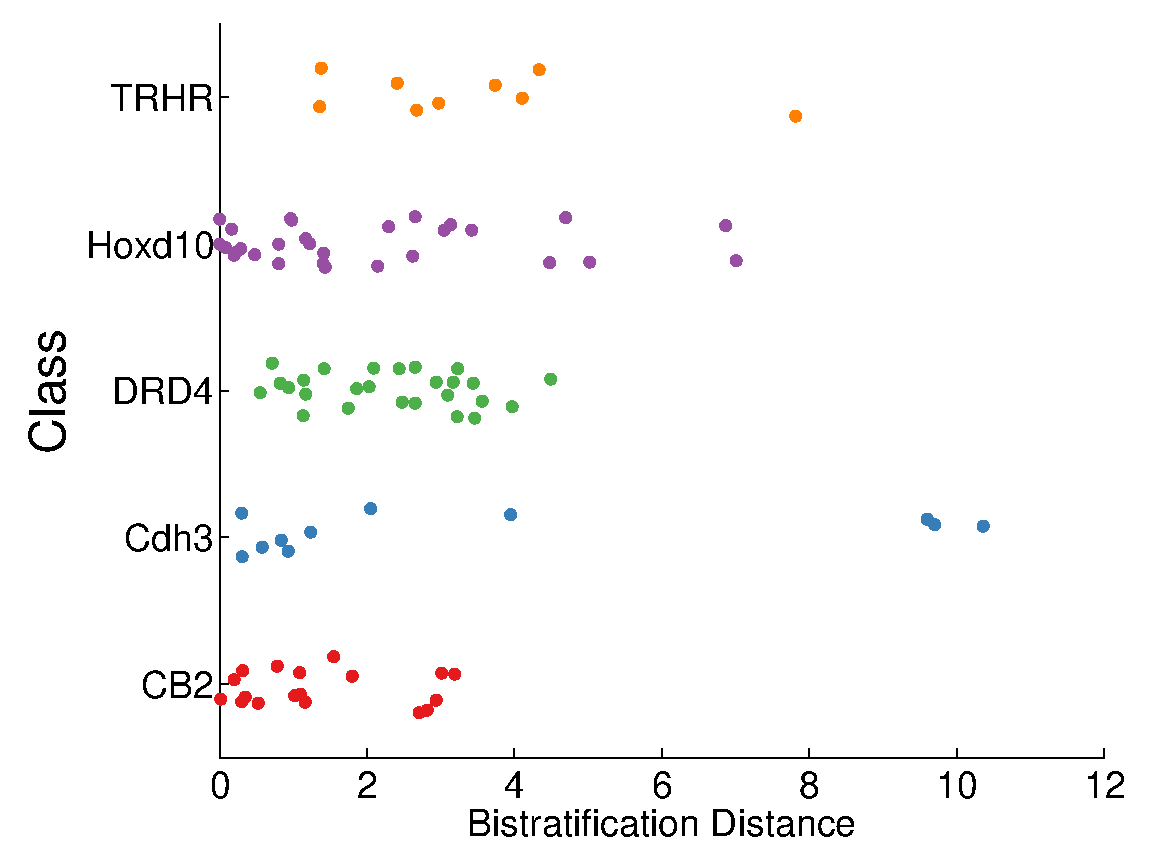
\includegraphics[scale=0.5]{Figures/SupFig3/plotFeatures-biStratificationDistance.eps}}
  \fbox{\includegraphics[scale=0.5]{Figures/SupFig3/plotFeatures-branchAssymetry.eps}}
  \fbox{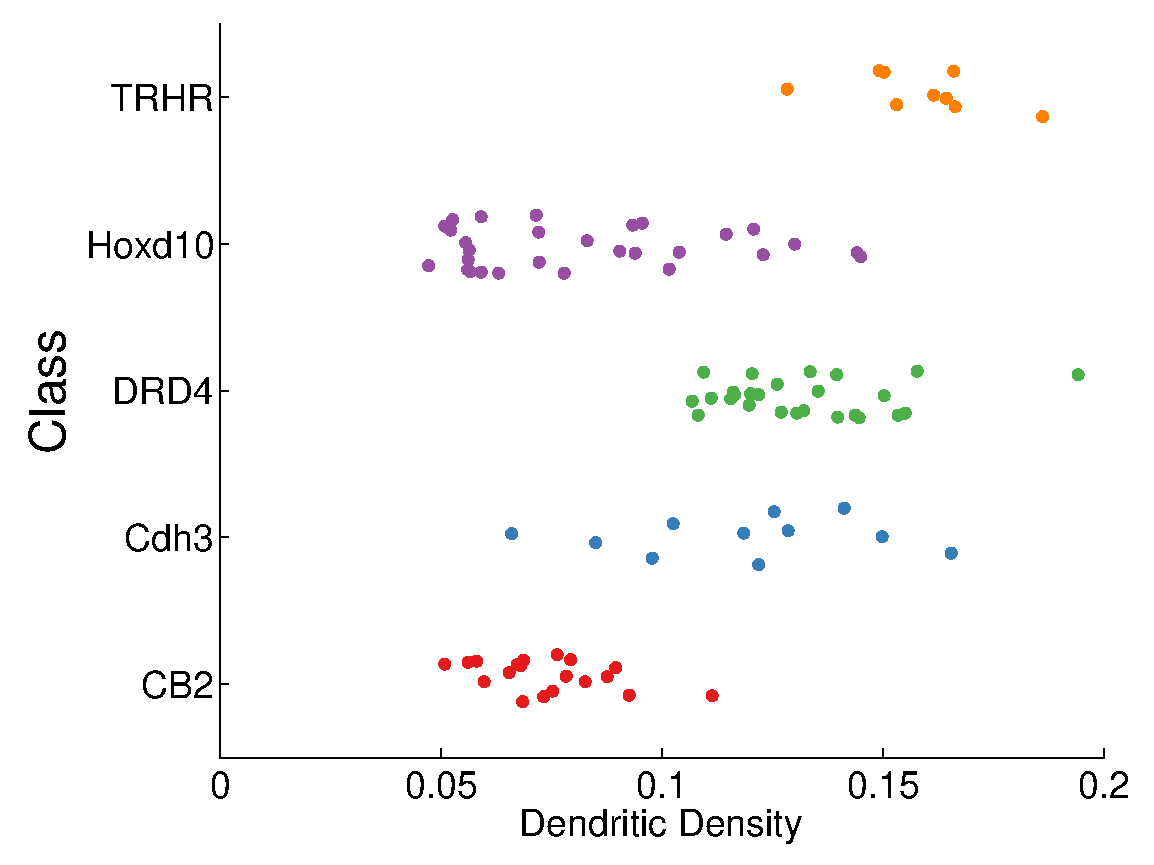
\includegraphics[scale=0.5]{Figures/SupFig3/plotFeatures-dendriticDensity.eps}}
  \caption{}
\end{figure}

\clearpage

\begin{figure}
  \centering
  \fbox{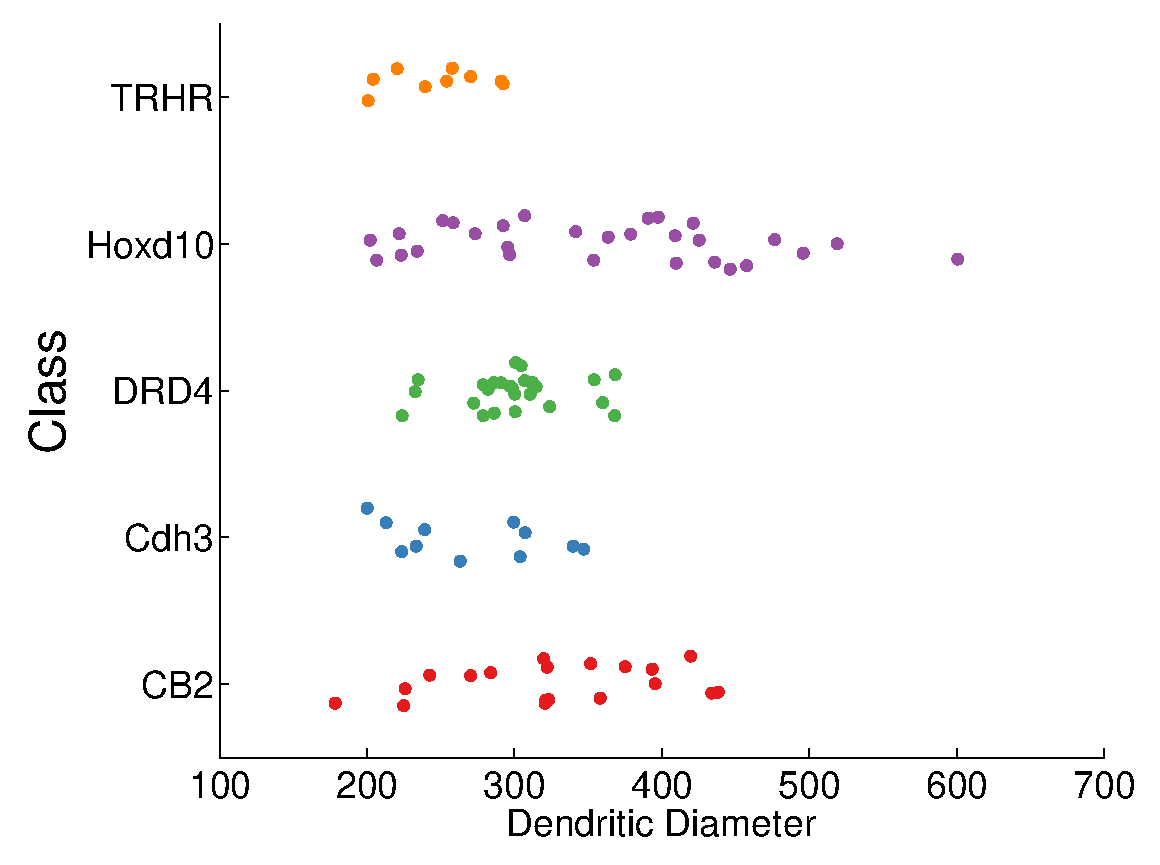
\includegraphics[scale=0.5]{Figures/SupFig3/plotFeatures-dendriticDiameter.eps}}
  \fbox{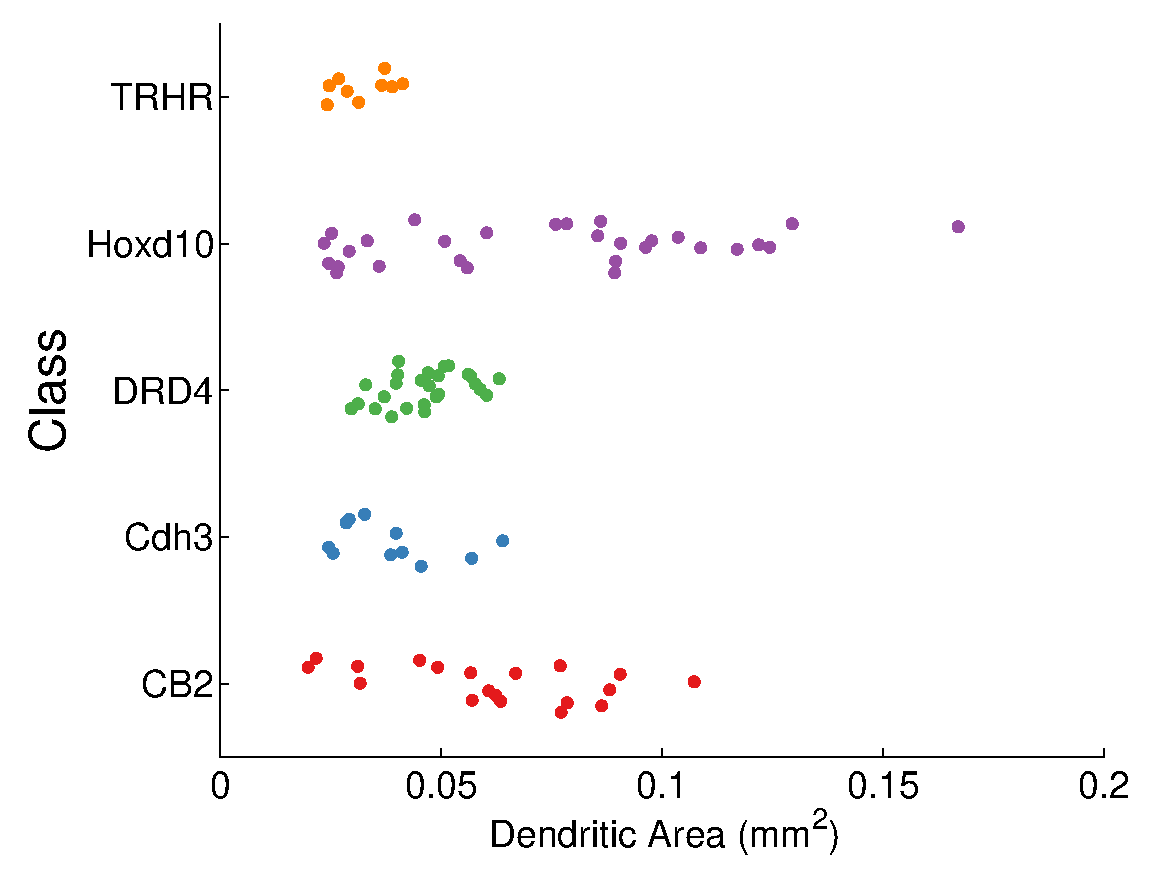
\includegraphics[scale=0.5]{Figures/SupFig3/plotFeatures-dendriticField.eps}}
  \fbox{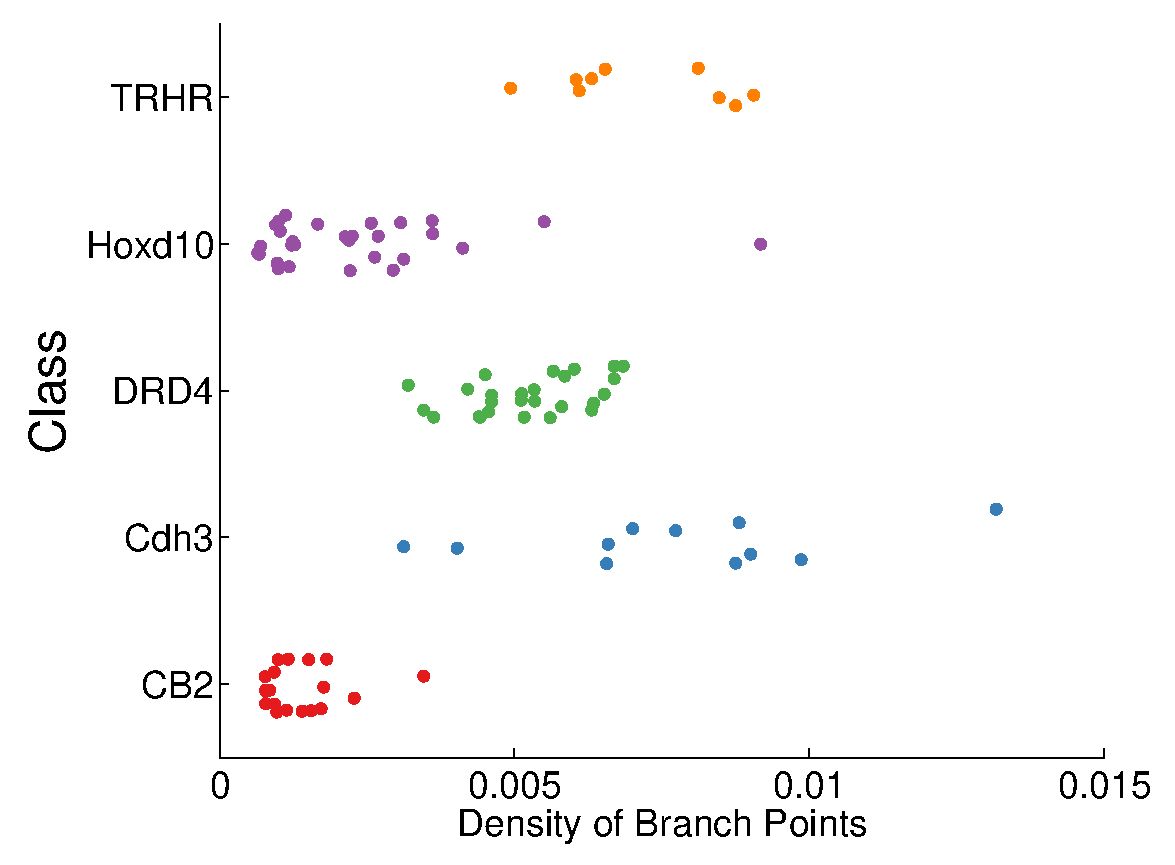
\includegraphics[scale=0.5]{Figures/SupFig3/plotFeatures-densityOfBranchPoints.eps}}
  \caption{}
\end{figure}

\clearpage

\begin{figure}
  \centering
  \fbox{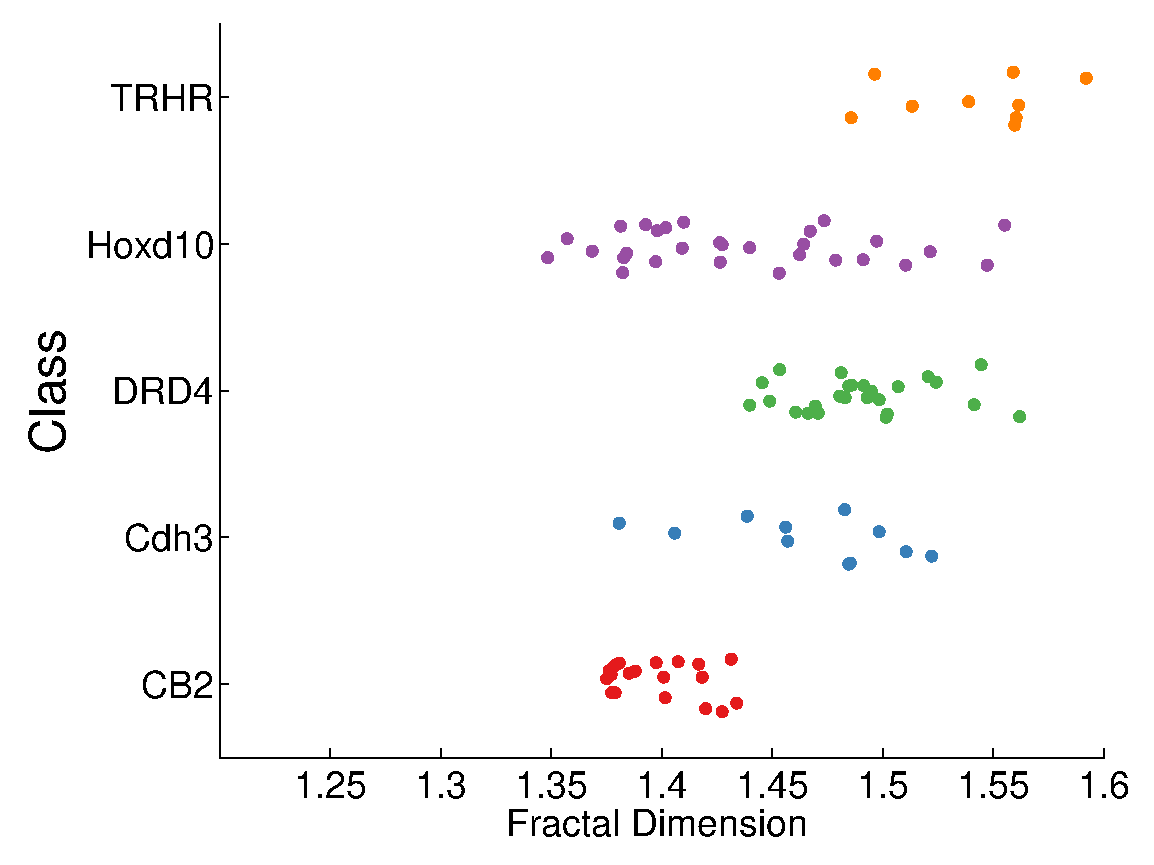
\includegraphics[scale=0.5]{Figures/SupFig3/plotFeatures-fractalDimensionBoxCounting.eps}}
  \fbox{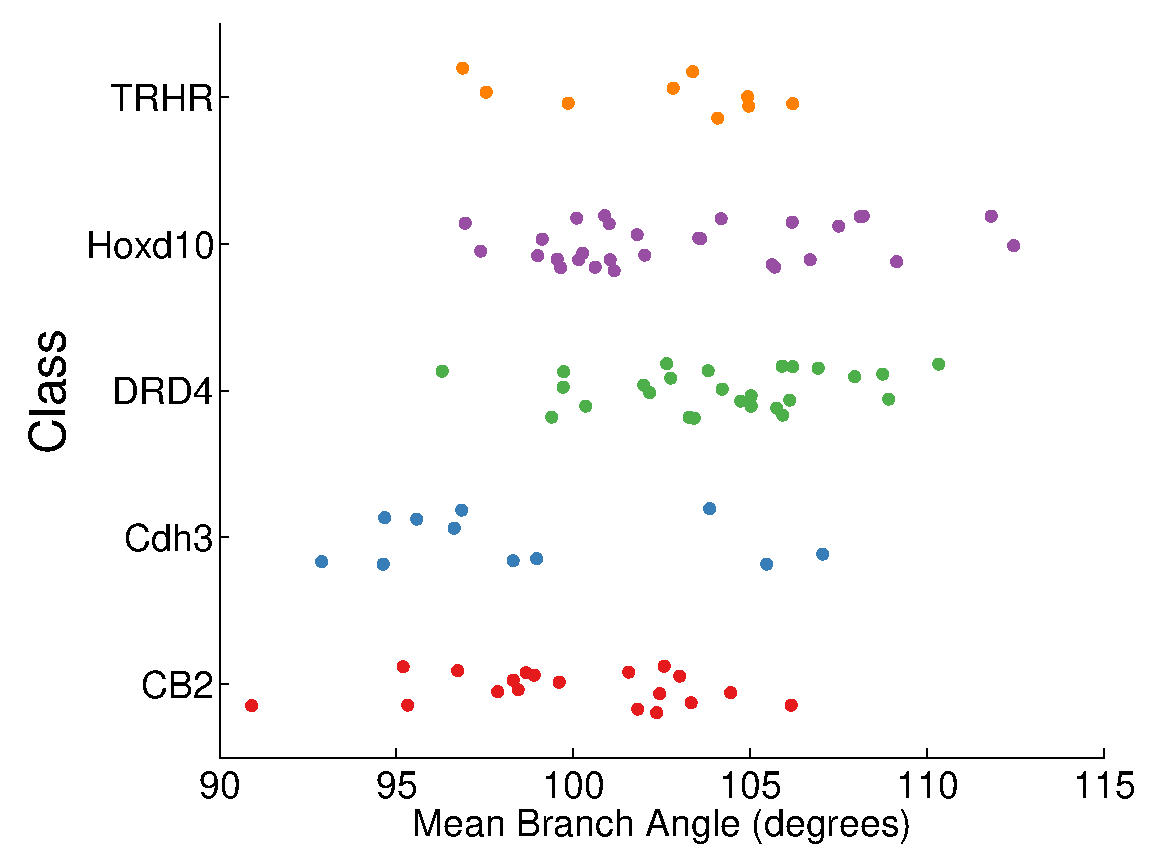
\includegraphics[scale=0.5]{Figures/SupFig3/plotFeatures-meanBranchAngle.eps}}
  \fbox{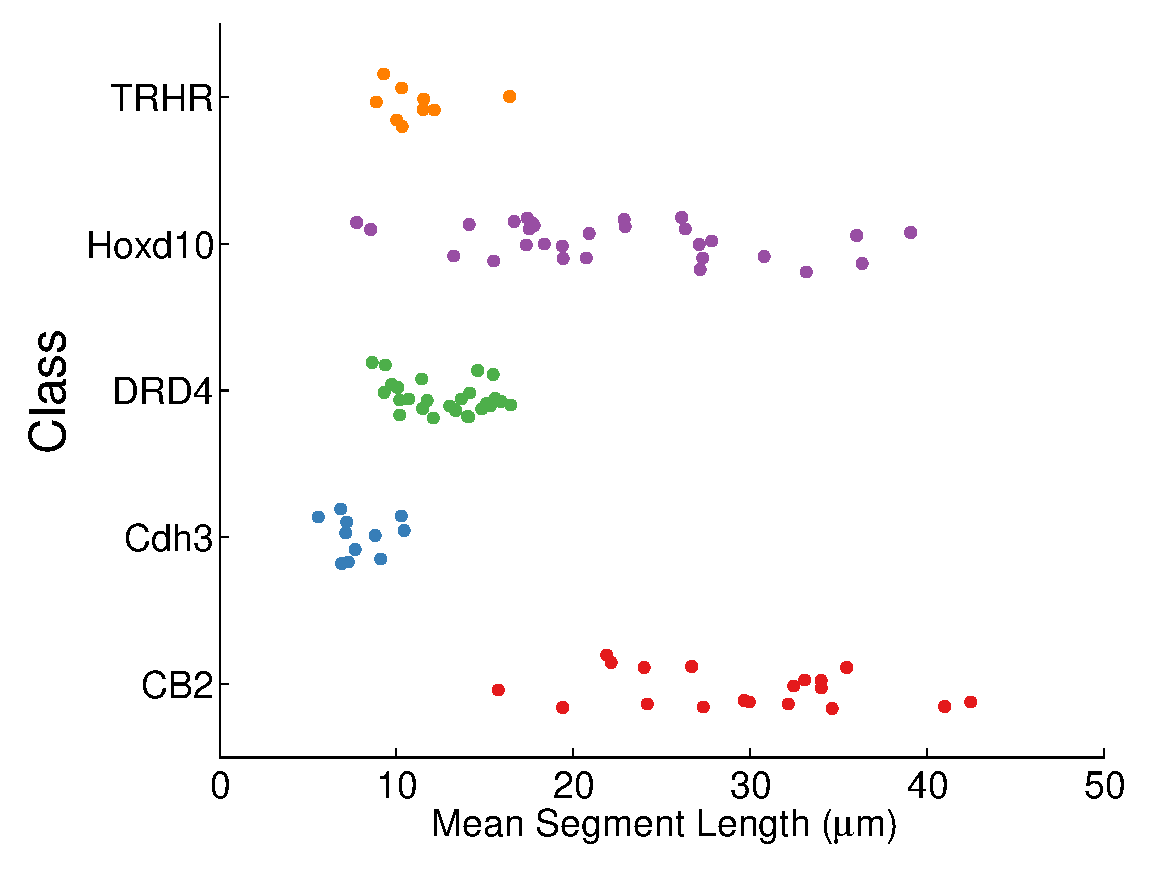
\includegraphics[scale=0.5]{Figures/SupFig3/plotFeatures-meanSegmentLength.eps}}
  \caption{}
\end{figure}

\clearpage

\begin{figure}
  \centering
  \fbox{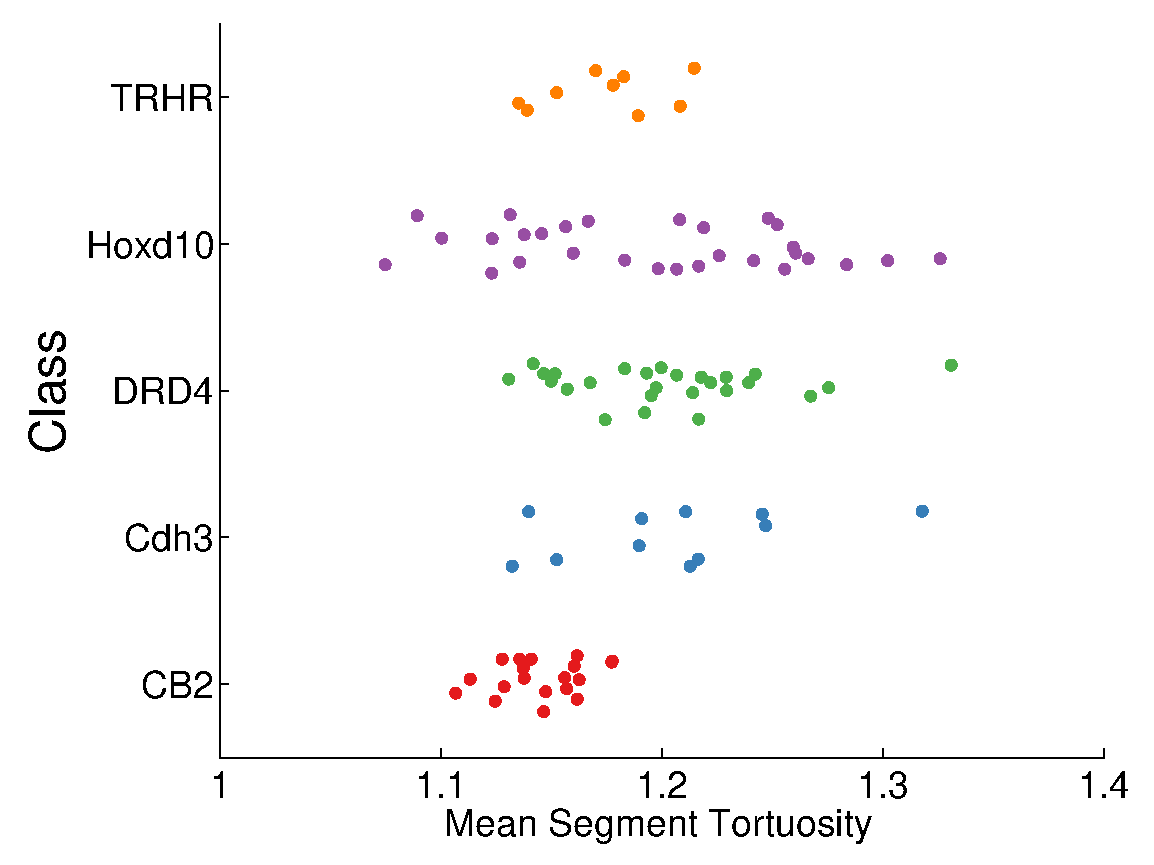
\includegraphics[scale=0.5]{Figures/SupFig3/plotFeatures-meanSegmentTortuosity.eps}}
  \fbox{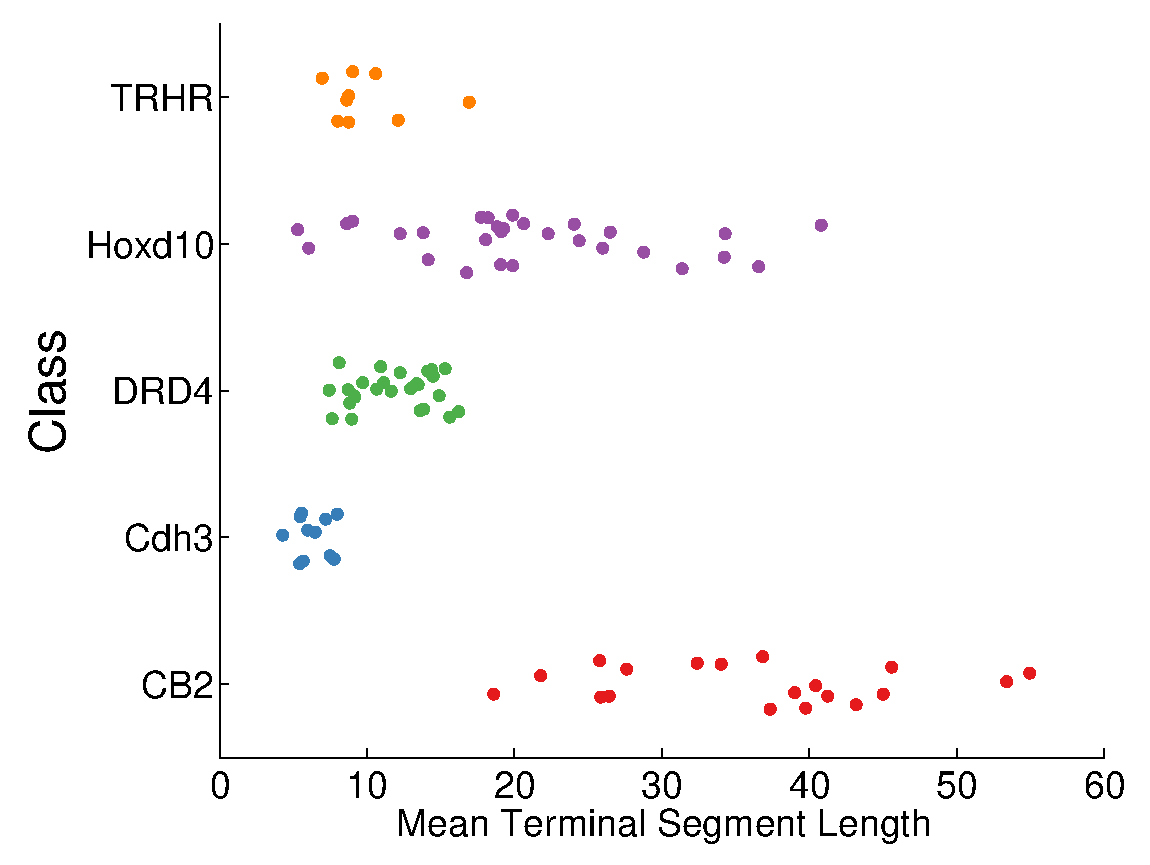
\includegraphics[scale=0.5]{Figures/SupFig3/plotFeatures-meanTerminalSegmentLength.eps}}
  \fbox{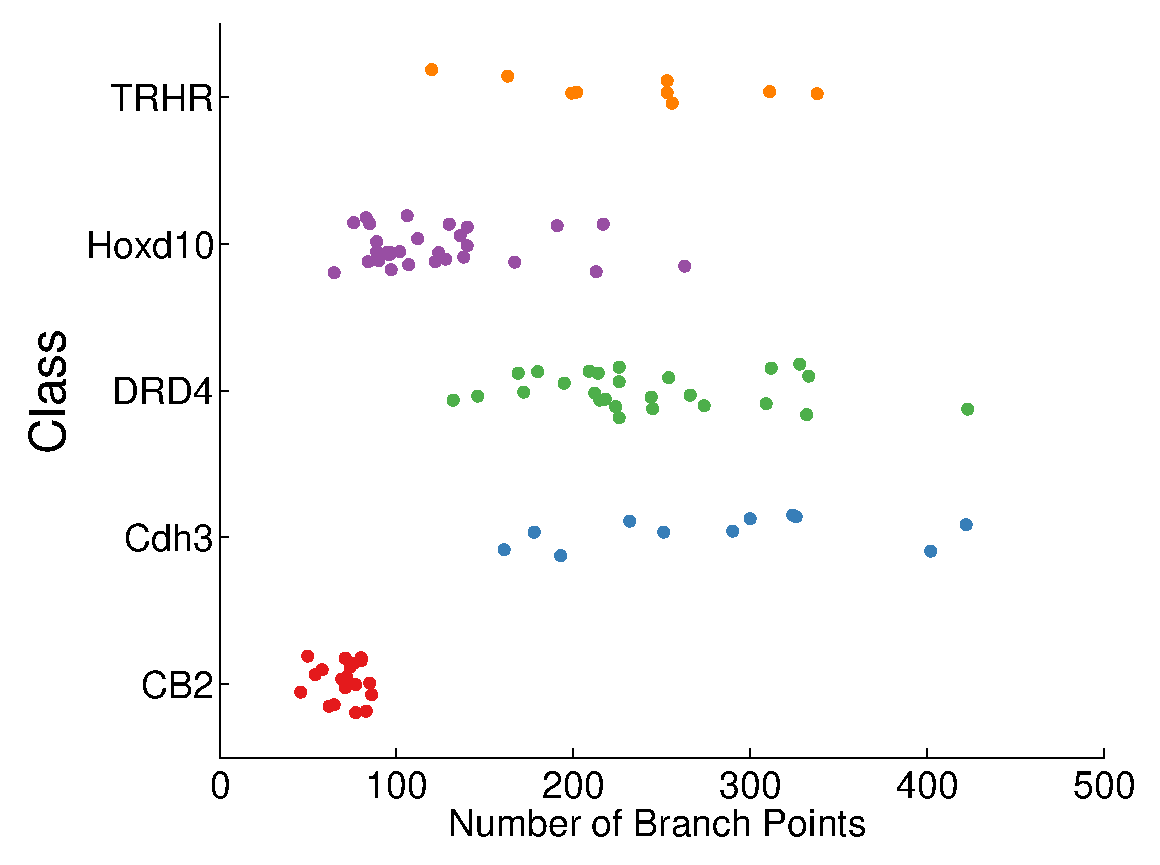
\includegraphics[scale=0.5]{Figures/SupFig3/plotFeatures-numBranchPoints.eps}}
  \caption{}
\end{figure}

\clearpage

\begin{figure}
  \centering
  \fbox{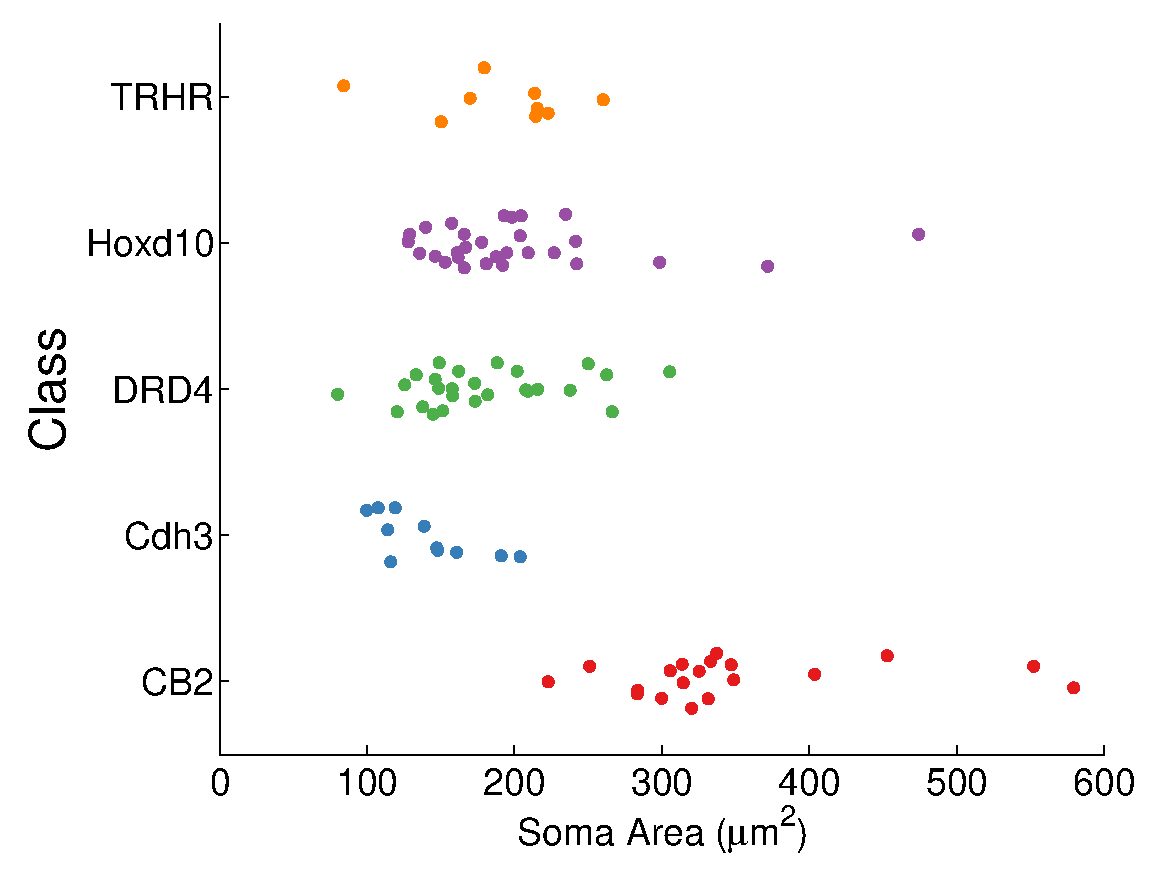
\includegraphics[scale=0.5]{Figures/SupFig3/plotFeatures-somaArea.eps}}
  \fbox{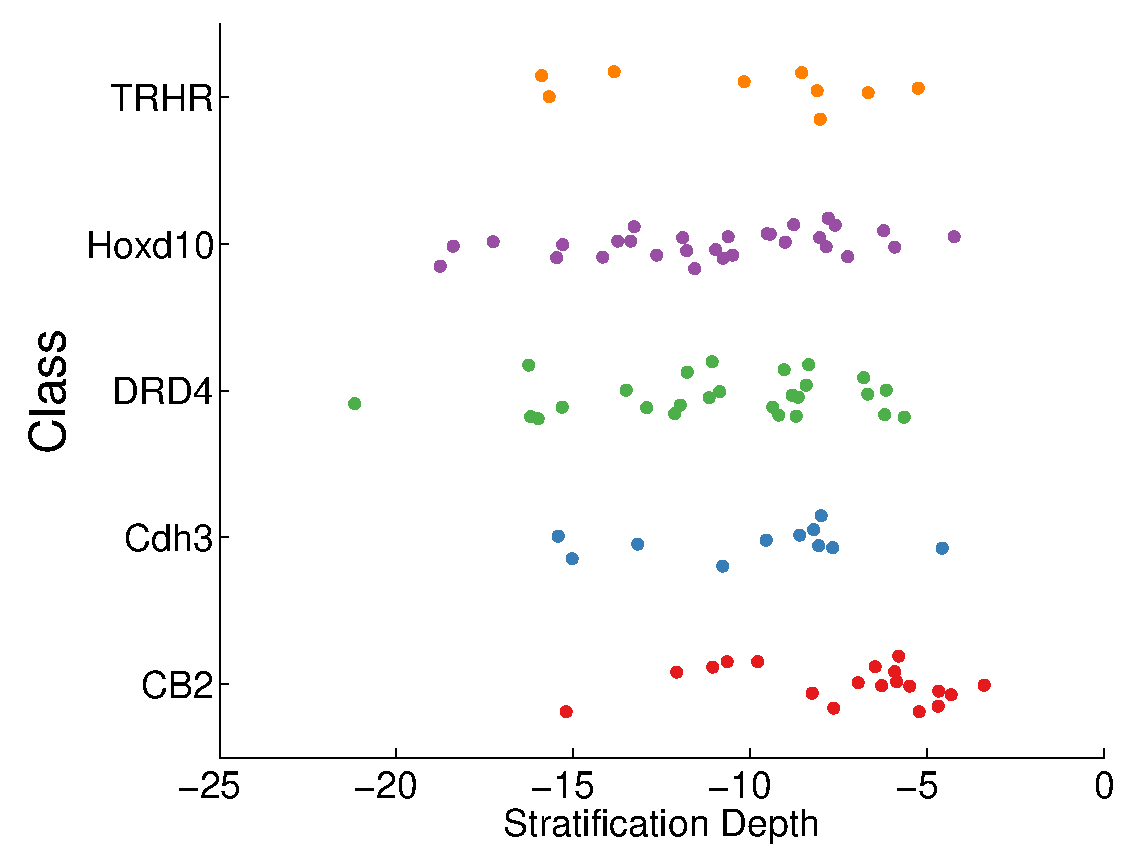
\includegraphics[scale=0.5]{Figures/SupFig3/plotFeatures-stratificationDepth.eps}}
  \fbox{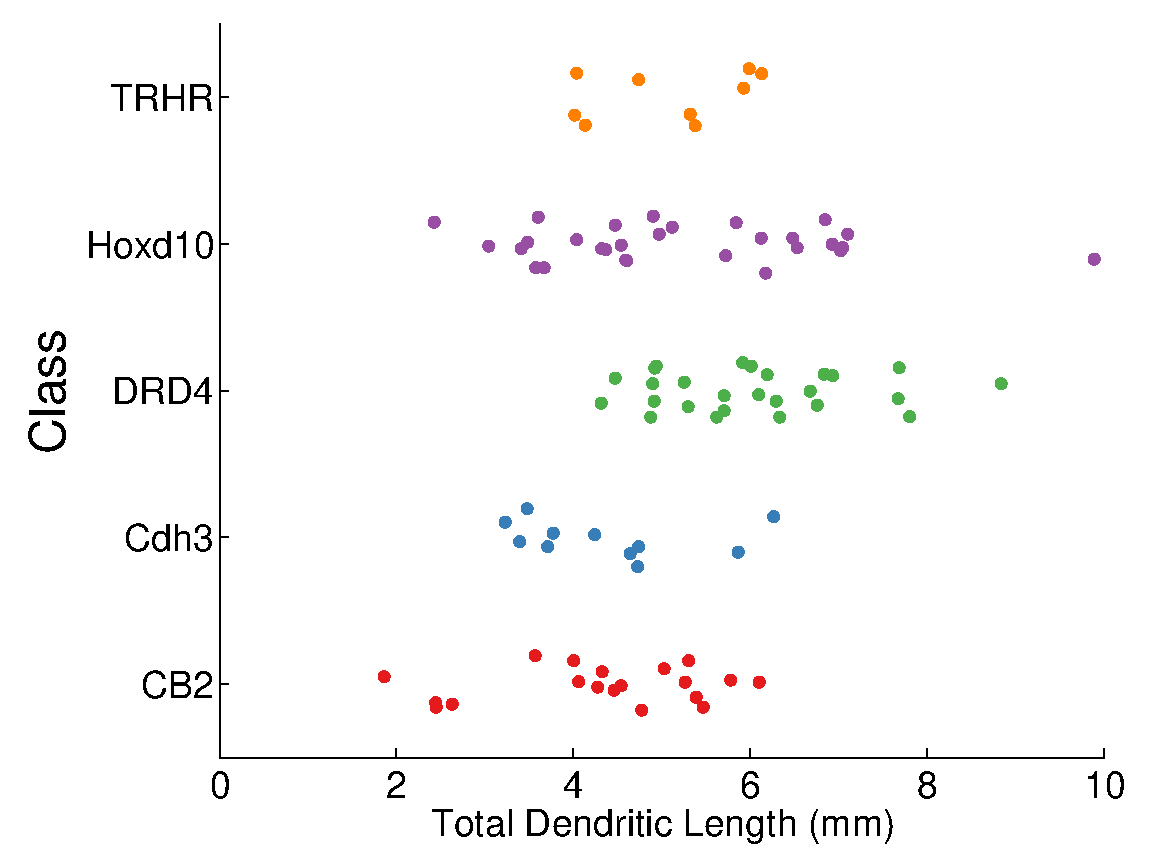
\includegraphics[scale=0.5]{Figures/SupFig3/plotFeatures-totalDendriticLength.eps}}
  \caption{}
\end{figure}

\clearpage



\end{document}
